%to have line numbers
%\RequirePackage{lineno}
\documentclass[10pt, letterpaper]{article}      
\usepackage[margin=.1cm,font=small,labelfont=bf]{caption}[2007/03/09]
%\usepackage{endnotes}
\usepackage{setspace}
\usepackage{longtable}                        
\usepackage{anysize}                          
\usepackage{natbib}
%\bibpunct{(}{)}{,}{a}{,}{,}                   
\bibpunct{(}{)}{,}{a}{}{,}                   
\usepackage{amsmath}
\usepackage[pdftex]{graphicx}  %[pdftex]git latex doesn't like it             
\usepackage{epstopdf}
\usepackage{hyperref}                             % For creating hyperlinks in cross references


% \usepackage[margins]{trackchanges}

% \note[editor]{The note}
% \annote[editor]{Text to annotate}{The note}
%    \add[editor]{Text to add}
% \remove[editor]{Text to remove}
% \change[editor]{Text to remove}{Text to add}



\marginsize{2.5cm}{2.5cm}{1.5cm}{1.5cm}%{left}{right}{top}{bottom}   
					          % Helps LaTeX put figures where YOU want
 \renewcommand{\topfraction}{1}	                  % 90% of page top can be a float
 \renewcommand{\bottomfraction}{1}	          % 90% of page bottom can be a float
 \renewcommand{\textfraction}{0.0}	          % only 10% of page must to be text

 \usepackage{float}                               %latex will not complain to include float after float

\usepackage[table]{xcolor}                        %for table shading
\definecolor{gray90}{gray}{0.90}
\definecolor{orange}{RGB}{255,128,0}

\renewcommand\arraystretch{.9}                    %for spacing of arrays like tabular

\newenvironment{ig}[1]{
\begin{center}
 %\includegraphics[height=5.0in]{#1} 
 \includegraphics[height=3.3in]{#1}
\end{center}}

 \newcommand{\cc}[1]{
\hspace{-.13in}$\bullet$\marginpar{\begin{spacing}{.6}\begin{footnotesize}{#1}\end{footnotesize}\end{spacing}}
\hspace{-.13in} }

\usepackage{datetime}


%\usepackage[latin1]{inputenc} %git latex compiler doesn't likeit
\usepackage{tikz}
\usetikzlibrary{shapes,arrows,backgrounds}


%\usepackage{color}					% For creating coloured text and background
%\usepackage{float}
\usepackage{subfig}                                     % for combined figures

\renewcommand{\ss}[1]{{\colorbox{blue}{\bf \color{white}{#1}}}}
\newcommand{\ee}[1]{\endnote{\vspace{-.10in}\begin{spacing}{1.0}{\normalsize #1}\end{spacing}\vspace{.20in}}}




\usepackage{sectsty}
\allsectionsfont{\normalfont\sffamily}



\usepackage{sectsty}
\allsectionsfont{\normalfont\sffamily}
%\usepackage[margins]{trackchanges}

\renewcommand\familydefault{\sfdefault}

\usepackage{verbatim}
\usepackage{rotating}
\usepackage{catchfilebetweentags}
%-------------------- END extra options -----------------------------------------
\date{Draft: {}\today}
\title{ % {\small Classification: Social Sciences}\\
%  
%  The Paradox of Energy Consumption and Happiness Across Countries
%Presonal 
Energy Use And Happiness% \footnote{Author Contributions:$<$blind for peer review$>$
  % AOK and MA designed
  % research. AOK. performed research. AOK. analyzed data. AOK and
  % MA wrote the paper.
  % Micah: Add author contribution statements. See: http://www.nature.com/news/publishing-credit-where-credit-is-due-1.15033
%}
}
\author{
% Adam Okulicz-Kozaryn, Corresponding Author, Department of Public Policy\\ Rutgers, The State University
% of New Jersey, Camden Campus\\ 401 Cooper St Camden NJ 08102\\(856) 225-6353; adam.okulicz.kozaryn@gmail.com
}

% \thanks{EMAIL: adam.okulicz.kozaryn@gmail.com
%   \hfill % I thank XXX.  All mistakes are mine.
% } \\
% {\small Rutgers, The State University of New Jersey, Camden}\\
% Micah Altman\thanks{EMAIL: micah.altman@gmail.com
%   \hfill } \\
% {\small Massachusetts Institute of Technology}


\begin{document}

%%\setpagewiselinenumbers
%\modulolinenumbers[1]
%\linenumbers

\bibliographystyle{/home/aok/papers/root/tex/ecta}

\maketitle
\vspace{-.4in}
\begin{center}
\end{center}

\begin{abstract}
\noindent  


It is widely claimed that there is a substantial tradeoff between energy
 preservation and human wellbeing. We are reluctant to cut energy
 consumption for fear of decline in our happiness. 
Despite technological advances, the Earth per capita energy use continues to grow.
The environmental consequences % of high rates of energy consumption
are well known:
resource depletion and pollution. % Is this avoidable?
%
 We study the relationship between energy consumption and happiness across four decades, and across multiple levels of geography.  Surprisingly, we find that received wisdom is false--for counties, states and nations, energy consumption is neither necessary for well-being, nor linked directly to it. 

%aok: i though we focus now too much on en intensity, and this is just one panel
%of one graph; the overall argument was about energy use in general

% We find instead that national well-being is strongly associated with the energy intensity of GDP. Although not a necessary condition for well-being, countries that efficiently convert energy to economic wealth, may benefit from increased energy use. 

% We lay out the possible causal explanations for differences in the energy intensity of GDP. Based on this we summarize the potential implications for designing policies that yield both high well-being and modest energy use. 
\end{abstract}


\vspace{.15in} 
\noindent{\sc keywords:  energy use,  energy consumption, energy intensity of economy, sustainability,  happiness, Subjective Well-Being (SWB)}
%\vspace{-.25in} 

\vspace{.15in} 


\begin{spacing}{1.0}
\rowcolors{1}{white}{gray90}

%  \ExecuteMetaData[../out/tex]{ginipov}

% \begin{figure}[H]
%  \includegraphics[height=3in]{../out/gov_res_trust.pdf}\centering\label{gov_res_trust}
% \caption{woo}
% \end{figure}

% Micah: 
%  Start with the strongest introduction we can possibly support. If we can't rigously support it with the data and analysis, we'll weaken it... but this is the goal. 
%  -- begin intro -- 

\section*{\large \bf Introduction} %energy policy requires such first heading

Environmental consequences of human consumption are the world's biggest
problems.  Energy consumption is a key component--the climate problem is an
energy problem \citep{mackay08}. For instance, 98\% of US emissions are due to
energy consumption \citep{eia08}. Despite
technological advances, the Earth per capita energy use has increased about 40\%
over past 40 years and it continues to grow. % (1890-1336)/1336
Most energy consumption both pollutes and  depletes natural resources
\citep{arrow04, soytas07}. %recent us: http://www.eia.gov/tools/faqs/faq.cfm?id=427&t=3 and
                          %for world even worst http://www.google.com/url?sa=t&rct=j&q=&esrc=s&source=web&cd=7&sqi=2&ved=0CDwQFjAG&url=http%3A%2F%2Fwww.iea.org%2Fpublications%2Ffreepublications%2Fpublication%2Fkeyworld2014.pdf&ei=uPMVVYaSM8OhgwSjqIKIAQ&usg=AFQjCNFX92MbI8lsvnDKqHCZqqoBnSMtSQ&sig2=NZpGqw3hDWdm3xcxvQyizA&bvm=bv.89381419,d.eXY&cad=rja  
 Energy consumption has, of course, many benefits as well.
 % MAYBE check these
% references if they are really to the point ! and possibly add some from goog
% drive folder
% Energy use and pollution are highly correlated, but they are not the same,  and
 The question remains about the net effect, how energy use affects human
 wellbeing on the whole.
 % we will differentiate between various types of energy use.  
We use a happiness yardstick
to evaluate benefits and problems of energy use. Traditionally, Gross Domestic
Product and its adjustments--per capita and purchasing power parity--have been
used to evaluate development \citep{jorgenson14C}. Human Development Index (HDI)
added life expectancy and education, but more recently a co-inventor of HDI,
Amartya Sen, has proposed happiness as better measure of overall development or
progress 
\citep{stiglitz09al}. 

% importantly there is spatail mismatch in resource demand and supply--notably
% china need a lot and has few; opec countries have oil; etc etc
%for instance recent emissions cap deal between US and China has largely to do
%with enrgy use e.g. http://mobile.nytimes.com/2014/11/13/opinion/climate-change-breakthrough-in-beijing.html?_r=0
It is universally acknowledged that there is a fundamental tradeoff between
societal energy preservation and individual self-interest. Substantially reducing
energy consumption requires individual sacrifices: If we reduce consumption, our
wellbeing will 
suffer \citep{gordon_wsj_may_29_14, dietz15, carter_pbs_apr_18_77,smil05}. %kenny_businessweek_aug_29_14, 
%COPIED FROM http://www.sciencedirect.com/science/article/pii/S0301421511001042
% The remarkable improvements in quality of life that occurred during the industrialization of Europe, North America and Japan in the 19th and early 20th centuries were caused, in large part, by the invention and adoption of energy intensive technologies (Smil, 2005). Coal was used to fuel steam engines, petroleum fed internal combustion engines, and all the fossil fuels plus falling water turned electrical generators.
%
%also, the point is that there is more popular wisdom instead! we know little scientifacally!hence our paper!
%
% and there is a Lancet series; but they did with health what we do with
% happiness:energy helps with health but also destroys it:
% http://www.sciencedirect.com/science/article/pii/S0140673607612537
% http://www.sciencedirect.com/science/article/pii/S0140673607612586
% http://www.sciencedirect.com/science/article/pii/S0140673607612525
% http://www.sciencedirect.com/science/article/pii/S0140673607612598
% http://www.sciencedirect.com/science/article/pii/S0140673607612550
%
%
% A very fundamental question is how to achieve both happiness and
% sustainability--it is difficult because there appears to be a tradeoff.
% Fundamentally,
%  the ultimate goal of increased energy consumption is human
%  happiness--if there is no relationship between the two, then we can
%  consume less and stay happy.
%
In this paper, we find that this universal assumption is wrong.  By combining
data on energy consumption and happiness we find that the
%relationship is weak at best. % , with exception of poor countries, where more energy is% nneded for greater happiness.
 people in areas consuming more energy are not happier.
This finding is robust across time, and multiple levels of spatial aggregation--it applies to patterns of energy consumption  at the local, national, and global scale.  


% -- end intro -- 

%Energy consumption matters.% beyond happiness
 Energy is a strategic
resource. Countries wage wars about energy sources  and much of politics is
driven by energy. % Many countries' whole economies depend on energy exports% , for instance OPEC countries.
Many  countries rely heavily on energy production
and some use it as a political tool. % , for instance, Russia.
%
 Virtually all countries  always seek to obtain more energy sources. A recent example is so called
fracking. Yet, we need to consume less. There are at least two
obvious reasons--most of energy consumed  is non-renewable and will stay
that way for some time \citep{mackay08}--most energy comes from
fossil fuels, which will run out. %MAYBE be specific give numbers
Second, energy consumption results in pollution, and pollution harms not only
 environment and other species, but also  humans, the beneficiaries of energy
consumption \citep{mackerron09,gandelman12,ferreira13}. Natural resource
depletion and pollution potentially cancel out the benefits of energy
consumption. 
 
A recent report by
Intergovernmental Panel on Climate Change is alarming 
(\url{http://www.ipcc.ch}). % very important body; another pnas citing it
                             % already in title http://www.pnas.org/content/104/24/10288.full
Indeed, a threat is serious enough that
claims for not growing the economy anymore or even ``degrowing'' 
appear reasonable \citep{kallis11, kallis12}. % \footnote{Although it is not
  % immediately obvious what is the best strategy to achieve greater
  % sustainability--degrowth \citep{kallis11} or simply public policy
  % \citep{bergh11}--for more discussion see \citep{daly13,kallis12}.}
At very
least curbing consumption is a reasonable course of action. Some argue reduction as high
as by factor of 10 in affluent societies \citep{pretty13}. This,
of course, begs a question, what would happen to our wellbeing?
 Again, a common % or received
wisdom is that there is a link between happiness and
energy use--happiness requires energy consumption.
Arguably, the very end goal (usually implicit)
of energy consumption is wellbeing or happiness, and hence,  % This is
% true in buivaraite case--the richer areas are happier.
%  We argue here that it is not necassarily so, only after taking into account
%  income at country level % and few other variables at state or county levels,
%  the relationship between energy consymptiona nd happiness disappears.
%
% its striking 2 fold or more differences between states like nj and tx and only a
% small fracton of that is due to climate most due to consumption arguably
% wateful/conspicous--calculate how mich explained by climate! give number
 energy conservation may result in happiness loss.
 We argue here that such loss, if
any,  will
not be substantial. Results suggest that curbing energy consumption that results
in pollution, i.e. most of today's energy use, will not affect adversely our
happiness in the developed world.  % There is anectodal evidence pointing to the fact that humans can
% live happily without much energy--among Amish, African Maasai, and Greenlandic
% Inughuit, most people are above neutral in well-being. \textbf{TODO cite!}


\section*{\large \bf Analysis and Results}

% Micah: This needs to be reorganized. 

% In my view the primary goal of this section is to answer this question:
%  *** Which choices do individuals make, that have a large negative effect on the environment, and which do not make the individuals, their community, or society better off?  ***
% We aim to provide the best scientifically and empirically supported answer possible, that does not require collecting new primary data. 


% AOK: another paper !
% this is interesting, probably more interesting than what we have so far, the
% problem is that we did not really test for that; now i was actually surprised
% that there are  data by census or climate
% regions (9 of them): 
% http://www.eia.gov/consumption/residential/data/2009/index.cfm?view=consumption
% and we have happiness there too: but you are asking a grand question; and the
% data we have just breaks down energy use in a big region estimating how much is
% used for cooling, heating, lights, etc etc--but there are a function of climate,
% culture and other collective stuff; for your question we would need person-level
% data and there are some (PSID for instance), but that's a different paper...

% what we have done so far is that there is not much happiness from energy use;
% probably much less than expected...

% and then we can say that given that we can cut energy consumptin and stay happy

% so yes in a sense we do answe your question--it is just not ``which choices''
% buty specifically less energy in general

% I suggest the following organization
%  1. Provide an easy to interpret figure showing happiness vs. energy consumption at the global level (nations), for a single time period. This should illustrate the general weakness of the relationship between happiness and energy consumption without controlling for anything. Discuss the substantive size of the raw - uncontrolled correlation
% 2. Now discuss the details of the measures. explain that (a) the energy
% consumption measures include only those that are under personal control, 

% AOK: all residential is personal control; but affected by climate etc--hence we
% have controls

% and (b) have a substantial effect on environment. Cite the literature as appropriate

% AOK ok, cool will trhow in lit here

% 3. Show that this relationship is durable -- introduce time-series data to show that this holds over significant time-scales

%AOK:by relationship i guess you mean happiness-energy use; but happiness is
%mostly flat over time; same energy use: in the rich countries mostly flat or
%increaing a little; in developing it increases;so won't be much there

% 4. Show that this relationship is not an accident of scale. Drill down to states, then counties within california, and show the relationship holds
% 5. Now discuss other possible explanations for these patterns (a) use these explanations to suggest convariates/confounders (b) show the results of controlling visually first, or with a simple table, (c) use a statistical model to ensure that the visual impressions are not misleading

% \section*{\large \bf Materials and Methods}
%boilerplate following
% http://www.pnas.org/content/109/49/19949.full.pdf  
% http://www.pnas.org/content/112/3/725.full.pdf
% http://www.pnas.org/content/109/25/9775.full.pdf
We use the most comprehensive data available at multiple levels of aggregation
and over-time. There is a consensus that the survey items that we use, are good
measures of subjective wellbeing \citep{diener09,oswald09w,stiglitz09al}.
 All happiness measures come from surveys representative of given areas. Such measures are reasonably valid and
reliable \citep{diener13b}. % , consistent and stable? or means same as valid, reliable?
One caveat is cross-cultural comparability \citep{diener03b}. % The cross
% country results that we report, however, show  strong relationship and it is very
% unlikely that the whole effect is due to measurement error. Furthermore,
 We mostly use data within the US. % LATER Energy measures  discuss their reliability, validity etc just google around.
We focus on simple relationships. Multivariate regressions are
discussed in the supplementary material. 



\textbf{Global Patterns.} We start by examining the relationship between energy
use and well-being across the world, at country level.  % --there is not much variation in happiness over
% time, and energy consumption in developed areas is quite flat, too. 
We use happiness data from World Database of Happiness
(\url{http://www1.eur.nl/fsw/happiness/hap_nat/nat_fp.php?mode=8}). 
  Happiness scale is based on multiple data sources and mostly measured with answers to
"All things considered, how satisfied are you with your life as a whole these
days?" on scale from 0="dissatisfied" to 10="satisfied." 
The measure of total per capita energy consumption comes from the World Bank
(\url{http://data.worldbank.org/indicator/EG.USE.PCAP.KG.OE}). All data were
averaged over 2000-2009 period. Data are plotted in figure \ref{couWvsLsEnePerGdp2}.
 %we use total and not residential
                                %electricity because across countries it is
                                %about energy intensive technologies of the
                                %whole economy, type of economy...,  not just households that
                                %determine QOL and happiness of people; within
                                %countries these ar emore or less constant and
                                %hence we can focus more on personal consumption
% 
%
% may also say that there are severalfold diff not only in income but also in ene
 The basis for the received wisdom that increasing well-being requires increased
energy consumptions is illustrated by the figure on the left: Across countries,
there is a clear positive association between energy use and
happiness. Happiness generally increases with energy consumption, but the variance across
countries is large and there are many outliers. Some high energy use countries, such as
Russia (RU),  are unhappy. Many countries such as Costa
Rica (CR) or  Mexico (MX) are able to reach the highest level of happiness while maintaining very low energy use. 
%
% 4/13
% TODO--DONE?
%
% Fig 1a - graphical emphasize high well-being/low energy countries--did above
% in text: CR, MX
% Fig 1a - do we really believe Mex, Guatemal and Colombia have higher well-being -- seems like WVS may be incompletely
%		   measuring this: yep, they're pretty happy there!
%
Moreover, the  countries that strongly contribute to the positive
relationship between energy consumption and happiness are the highly-developed
Nordic countries (DK, FI, NO, SE). They have both unusually high energy use and
happiness. In general, developed countries have greater quality of life and
well-being \citep{mazur11, jorgenson14C}: How does the relationship between
energy use and happiness change if we take economic development into account?
% 4/13
% TODO--DONE? i rephrazed question to simplify to what we are doing here;
% answering the original question would be more for a book or lengthy article 
%
% Is the attribution to Nordic countries correct?
% Can we answer the question, at least partially?
% sure there is a lot of other things predicting happiness! Scandinavia uses a
% lot of energy because it is freezing there, and it is arguably v happy due to
% great governance, welfare, nature, low density etc etc

Surprisingly,  we find that when we measure energy as as a function of economic
efficiency, the relationship reverses.  This is shown in the second panel of
figure \ref{couWvsLsEnePerGdp2}, which displays on the x axis the energy intensity of gross domestic product (energy/GDP). Countries that consume less energy per unit of wealth are happier. 
%
In a descriptive sense, high energy intensity means that a country requires
a high cost to convert energy into GDP. Another way to put this is that some
countries are more efficient (in the economic, not technical sense) at
converting energy into wealth. There are a number of possible causal explanations.  Countries with lower energy intensity  use
 more energy-efficient technologies--these technologies reduce energy input 
for the same output of goods or services and consumption can remain high at low
levels of pollution.
% can elaborate a bit if needed better efficiency--less pollution per consumption--more good stuff without the bad stuff
%was thinking about how to neutralize too happy COL and few others, but it is
%what it is,may explain this a bit in text perhaps--e.g. see http://www.huffingtonpost.com/2013/01/17/reasons-colombia-happiest-country_n_2490813.html
 For instance,  the Netherlands (NL) is rich,  energy efficient and happy. But
 there are also outliers, for instance,  Colombia (CO) is  happy and energy
 efficient,  but poor.  
In general, Latin America poses a puzzle for happiness researchers. Latinos are
relatively poor but happy. Latinos also use very little  energy and have similar energy intensity to that of the  US. Notably, all Latin
 American countries cluster at the top left in the
first panel.  Great happiness is possible using little  energy. East European
post-Soviet countries, on the other hand, cluster at the bottom and some at the
left. Some countries are relatively unhappy despite low energy intensity of GDP such as Congo (CG). Some countries, on the other hand, are relatively happy
despite high energy intensity such as Trinidad and Tobago (TT) and Kazakhstan (KZ).    
% also see http://www.ritholtz.com/blog/2010/06/oil-consumption-around-the-world/ 
\begin{figure}[H]
 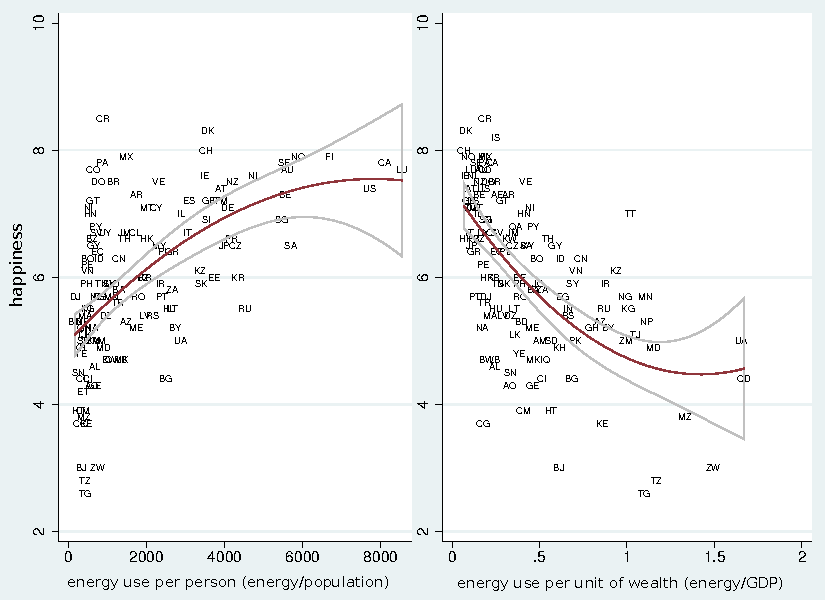
\includegraphics[width=6in]{graphsAndTables/couWdhEneGdp--inkscapeEdited.pdf}\centering \caption{Countries
   that consume more energy per person are happier (first panel), but countries
   that consume more energy per unit of wealth are less happy (second
   panel). Positive relationship in first panel is spurious--taking into
   account level of development, the relationship reverses. 
Quadratic fit shown with 95\%  confidence intervals. Energy use
   refers to use of primary energy before transformation to other end-use
   fuels. All data were averaged over 2000-2009 period.  % For average electricity consumption per electrified household, which shows a similar picture, see figure \ref{couWvsLsEleHHgdp} in supplementary material.
% For graphs using happy life years as a dependent variable see graph \ref{hly} in
% supplementary materials.
 Country codes are in table \ref{ls} in supplementary material. 
 Several outliers were dropped: countries with energy use above 10,000: United Arab Emirates, Iceland, Kuwait, Qatar, Trinidad and Tobago; and countries with energy intensity higher than 2: Ethiopia, Turkmenistan, Uzbekistan.}\label{couWvsLsEnePerGdp2} 
\end{figure}
% \begin{figure}[H]
%  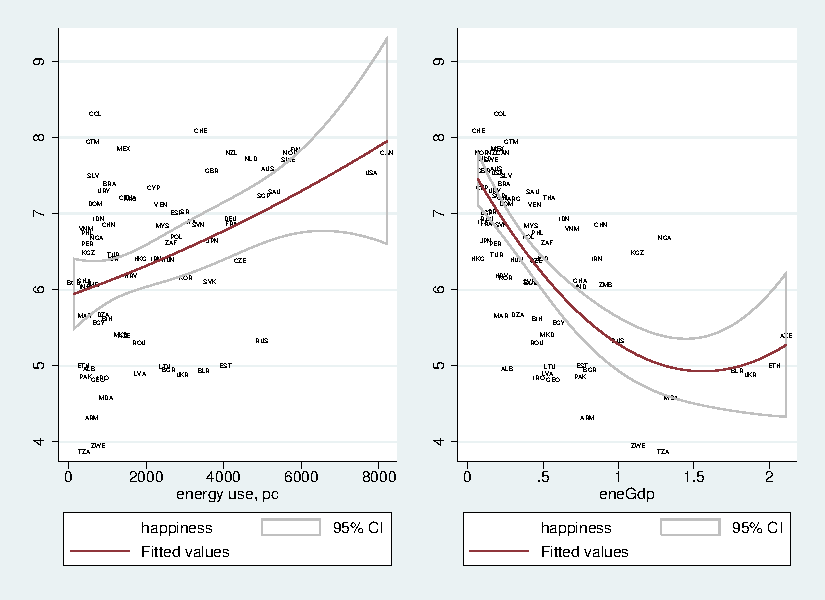
\includegraphics[width=6in]{graphsAndTables/couWvsLsEnePerGdp2.pdf}\centering \caption{Happiness
%    against GDP, total energy use, and energy intensity of GDP. Quadratic fit
%    shown with 95\% confidence intervals. Happiness is measured with "All things considered, how satisfied are you with your life as a whole these days?" on scale from 1="dissatisfied" to 10="satisfied." Energy use refers to use of primary energy before transformation to other end-use fuels, which is equal to indigenous production plus imports and stock changes, minus exports and fuels supplied to ships and aircraft engaged in international transport. For average electricity consumption per electrified household, which shows a similar picture, see figure \ref{couWvsLsEleHHgdp} in supplementary material.  Note: Country codes are in table \ref{ls} in supplementary material. We use a cumulative file covering first four waves, 1981-2007. If country was observed in more than one year, data were averaged.}\label{couWvsLsEnePerGdp2} %couWvsLsEnePerGdp2 doesn't have gdp only; couWvsLsEnePerGdp2 adds gdp as first panel
% \end{figure}


% In poor countries more income and sometimes more energy may be beneficial to human
%  wellbeing. In rich countries, on the other hand,  it is likely that not only we do not need
% more energy, but also, arguably we should consume less energy \citep{mazur74}. There are even
% calls to stop growing income in rich countries or even degrow it
% \citep{kallis11,kallis12,bergh11}.
\textbf{US States and Counties.} We turn to the US in an effort to answer
an old question of whether more energy is needed to increase wellbeing if there
is already a great deal of energy being consumed \citep{mazur74}. The US is among
countries using most energy per capita.
% Also, we focus
% now on electricity consumption because it is representative of modern
% energy %niu13 
% and it is growing fast. %winfrey13 p7
% electricity for CA only--can add this explaation + lack of total energy use i
% guess if reviewers compalin about electricity in california! 
%

State and county level happiness data come from the Behavioral Risk Factor
Surveillance System (\url{http://www.cdc.gov/brfss}) using a similar happiness question: ``In general,
how satisfied are you with your life?'' on scale 
from 1=''very dissatisfied'' to 4=''very satisfied.'' State energy  data come from
US Energy Information Administration (\url{http://www.eia.gov/state})  and is measured as total energy
consumption per capita in the residential sector.  
California's  residential electricity consumption per capita come from 
Energy Consumption Data Management System
(\url{http://www.ecdms.energy.ca.gov/elecbycounty.aspx}). State level data are
averaged over 2005-2010, and California data are
averaged over 2006-2010.
Results are shown in
figure \ref{stateCaPAP}. Energy-hungry states  are not happier. % --this is just another argument for energy conservation
% (with possible exception of transportation sector) commented out--this was
% confusing-we do not show transpo sector here
 There are two outliers, Hawaii and California, consuming much less energy in
the residential sector than others. 

We zoom in on California counties in
second panel of the same figure. There is also a great deal of variation in energy
use across California counties, and the relationship with happiness is nil. 
% So California consumes only about half of the energy consumed by an average
% state.  also see http://www.skepticalscience.com/print.php?n=1365
We have  experimented with energy intensity of
GDP as we did earlier across countries, but in case of the US subregions the results are
not different. %supplemnetart material picture XXX

%MAYBE can make it flatter as fig 1 so that subgraphs are square
\begin{figure}[H]
 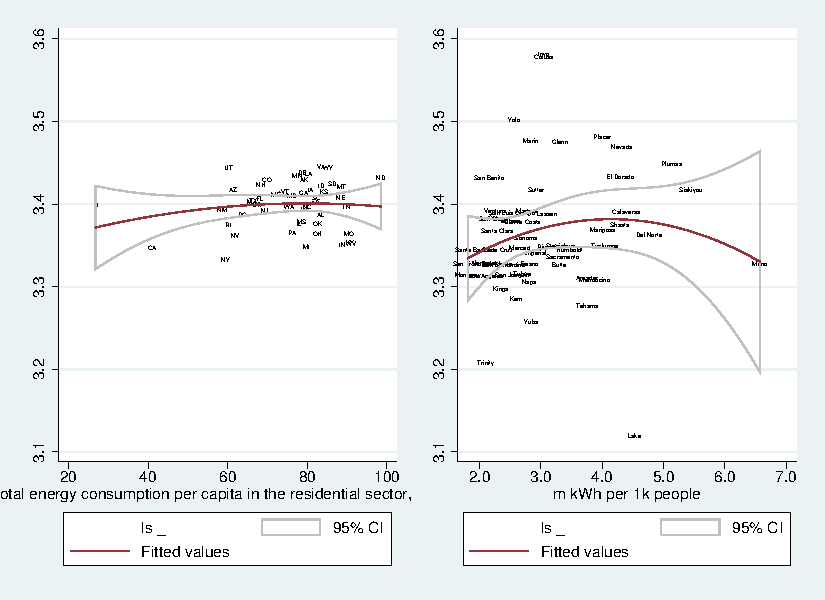
\includegraphics[width=6in]{graphsAndTables/stateCa.pdf}\centering
\caption{Happiness and total residential energy use across US states and
  residential electricity use across   
  California counties.  % Happiness is measured with ``In general, how satisfied
%   are you with your life?'' on scale from 1=''very dissatisfied'' to 4=''very
%   satisfied.'' State energy use data come from
% U.S. Energy Information Administration and is measured as  total energy
% consumption per capita in the residential sector.  
% California's  residential electricity consumption per capita come from 
% Energy Consumption Data Management System
% (\url{http://www.ecdms.energy.ca.gov/elecbycounty.aspx})
 The relationship was also quite flat in terms of total energy consumption and
 its GDP intensity. State level data are averaged over 2005-2010, and California data are averaged over 2006-2010.
% --see figure \ref{lfTETPBgdpLS}
  % in supplementary material.
}\label{stateCaPAP}
 \end{figure} % {\scriptsize Note: Country codes are in table \ref{ls} in
              % supplementary material. If country was observed in more than one
              % year, the data were averaged. }%PNAS readership should know US
              % state codes!

{\bf Over Time Movement.} It is well-known that happiness is related to income
in  a 
cross-section, but not over time \citep{easterlin74,easterlin12}. We
supplement our cross-sectional results with an exploration over time. We use General
Social Survey (\url{http://gss.norc.org}).   %should be representatve %of regions but couldnt find any specific %evidence of that!
Happiness question reads "Taken all together, how would you say things are
      these days--would you say that you are very happy, pretty happy, or not
      too happy?" 1=''not to happy'', 2=''pretty happy'', 3=''very happy''. 
 Energy consumption is measured as total energy use per capita in
residential sector, the same measure as used for states. 
Figure \ref{cenDivLsYrSm} shows happiness and energy use over time by
census division. There is not much co-movement: the two series correlate at
.2 only. Energy consumption is only weakly related to happiness. 

\begin{figure}[H]
 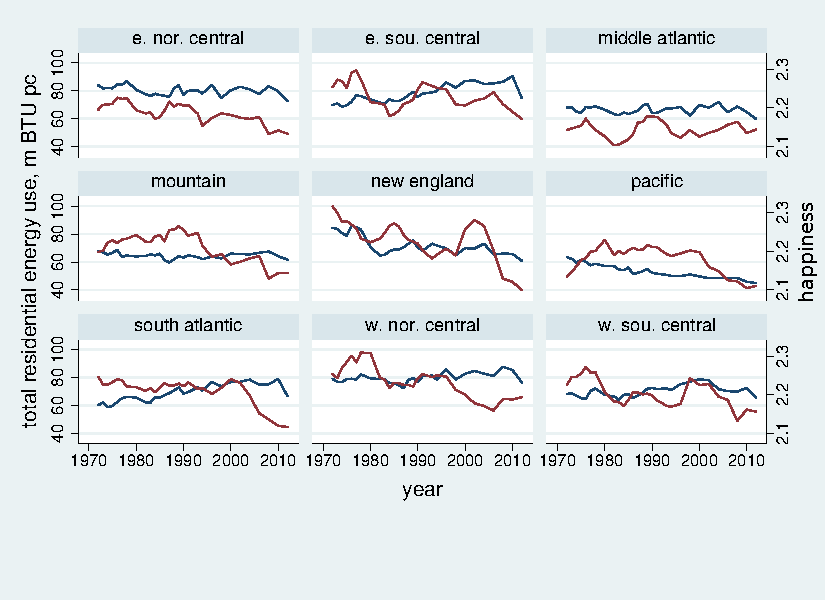
\includegraphics[width=5in]{graphsAndTables/cenDivLsYrSmINKSCAPE.pdf}\centering
\caption{Happiness (6-yr moving average) and total energy consumption
  in residential sector per capita. Correlation is .2 only (for unsmoothened series).
 % (for  unsmoothened series) for unsmotthened happiness see figure \ref{cenDivLsYr} in
 %  supplementary material.
  % Across countries there is not much variation in
  % happiness over time, neither in energy use--see figure \ref{ebTS} in
  % supplementary material.
}\label{cenDivLsYrSm}
\end{figure}

Americans continue to consume large amounts of energy as compared to other
countries.  With a notable exception of California, energy use is
not decreasing. % , and in some cases energy use has increased.
 Americans do not spend any less  on energy either: 5-10\% of personal
expenditure over past 50 years % , and if anything this amount
% has  increased slightly  over the last decade 
 \citep{bea-2-8-5}.
%   \url{http://burnanenergyjournal.com/what-goes-down-steins-law-and-the-cost-of-energy/}
% or \url{http://environmentalresearchweb.org/blog/energy-the-nexus-of-everything/}


%\section*{\large \bf Discussion}
\section*{\large \bf Conclusion and Policy Implications} %energy policy requires last sec to be labelled like this

% Micah: We'll rewrite this later. The main goal is to (a) briefly summarize the most significant results; (b) outline the possible causal explanations and frameworks, and thus define the future research agenda; (c) describe potential interventions 

% 4/13
% TODO--not sure what to do here--we do not really test them--do not have person
% level dataa and likely each contributes little explanation; so i just added in
% text that there can be many explanations and it is left for future research to
% find out which one:"This article only documents the relationship, and finding the cause is left for the future research--there are many potential explanations."
% This jumps traight to causal conclusions.
% Need to be very careful about evaluating the evidence for the explanations we propose:
%   - energy efficiency 
%   - hedonic treadmill
% 	- conspicuous consumption (not the same as treadmill)
%	- positional good consumption
%	- risk-homeostasis based consumption (bigger cars)
%	- comparative national advantage in energy-intensive industries
%	- different baseline requirements for climate 
%
% For each of these explanations
%    - can we rule them out (or is their strong evidence against them) in the current data
%	 - what type of observation would be needed to test them (what level of aggregation of people, type of energy use, over time, an do we need natural expderiment)
%	 - what are appropriate interventions
%	 - which  of the interventions increase well being w/out increasing energy use, using current current feasible tech?
%	 - which of the interventions can increase well being w/out increasing energy use, requiring tech?

At the country level,  the lower the energy consumption, given development
level, the happier the country.  Across US states and California counties,
energy consumption and happiness have a nil relationship. 
% it would be another reason for energy
% conservation.
Likewise, the over time changes in energy use are almost unrelated to changes in
 happiness across US Census regions. 
% These are important findings  because many assume that energy consumption makes us
% happy--this is presumably why we keep on consuming ever more energy and are
% reluctant to curtail this consumption.
% At the same time, there are important
% reasons to curtail the consumption.
With this correlational study we aim to bring the relationship between energy
use and wellbeing to wider audience, and encourage more research in this area. 

% Germany plans for renewable energy
% http://www.nytimes.com/2014/12/01/business/energy-environment/plan-outlines-low-carbon-future-for-germany-energy.html

Happiness can be achieved at low levels of
energy consumption. At high level of energy consumption, such as
that in the  US, energy and happiness have a nil relationship. % If developed world changes from society of consumers
% to society of conservers, we will not suffer much in terms of
% happiness, if at all.
 This finding is against a widely held assumption that the relationship is
positive. This discrepancy between expectation (more energy use, more happiness)
and experience (more energy use, not more happiness) is not necessarily
 surprising. A decision on how much energy to produce and consume is based on
 expected happiness. But humans are often predictably wrong and experience much
 less happiness than expected \citep{kahneman97ws}, and are wrong
 in their perceptions of energy consumption and savings \citep{attari10,dietz14B}. 

% \begin{figure}[H]
%   \begin{centering}
%     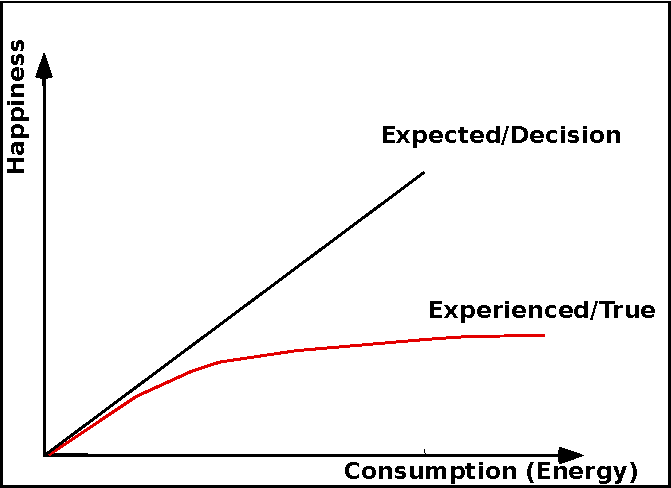
\includegraphics[height=2.0in]{graphsAndTables/utility}
%     \caption{Expected v experienced  happiness \citep{kahneman97ws}. Humans make
%        decisions about consumption based on expected or
%       decision happiness, but the experienced or true happiness tends to be 
%       lower than expected when greater consumption is achieved.}\label{fUT}
%   \end{centering}
% \end{figure}

In some developing countries more energy consumption may be needed to achieve greater happiness. In developed world, however, we
 arguably can decrease energy consumption without much loss in happiness, if any. % can alse give some numbers on how much energy uses an american v
            % chinese etc
Indians and Chinese may need to consume more energy, but not Americans. 
Texans, for instance,  could consume as much as Californians (they consume more than twice as
much). %http://www.eia.gov/state/rankings/
% Furthermore, it is unfair for the developed World to lecture developing
% countries about energy conservation without first making very substantial cuts
% at home.

Why energy use is unrelated to happiness, especially in developed nations such
as the US? This article only
documents the relationship, and finding the cause is left for the future
research--there are many potential explanations. Importantly, however, the
theory and potential explanations tend to predict our finding. 
Consumption beyond a point does not buy happiness. Such consumption buys
position, but because everyone tries to outcompete everyone else, this race
cannot be won. A related cause is a ``hedonic treadmill'' \citep{brickman78cj}:
Increased consumption does not necessarily increase well-being due to
hedonic adaptation. More consumption does not make people happy if basic needs
are already satisfied. %  Hence, there is
% a positive
% relationship between happiness and energy across countries, but the relationship
% in the US is nil.
% --poor countries need to consume more enrgy in order to increase their
% happiness, but not the rich countries
 A related explanation can be made using Veblen's concept of conspicuous or
 wasteful consumption \citep{veblen05a, veblen05b}. Such consumption does not
 satisfy needs but simply aims to demonstrate that
one is better than others. Much of such consumption wastes energy without
satisfying human needs, % , for
% instance, mansions and large cars.  Many other examples are not necessarily conspicuous, 
% but they waste energy and have no clear contribution to lasting happiness, for
% instance, much of landscaping including unnatural ponds, fountains, and other items that
% define American suburbia.
%
 and  does not make us any happier  \citep{csikszentmihalyi99, frank04, frank05,
   frank12}. % , but few actually test it.
  Even the popular claim that human wellbeing requires substantial energy use or
 the claim that there is a tradeoff between conservation and wellbeing are not
 well grounded in theory. According to the livability theory
 \citep{veenhoven14b}, more consumption does result in more wellbeing if it
 helps to satisfy human needs. Hence, energy used to alleviate extreme
 temperatures, provide food, shelter, basic transportation, etc, will increase
 human happiness (if it out-weights the costs such as pollution). But energy
 consumed on non-essential human needs (arguably most energy consumed in
 developed nations) will result in little happiness, if any, and this is what we
 find.  

% We complement our results % and again, the only  study testing the
% % effect of energy use on happiness was \citep{graef81}.
% %  Results suggests that  energy consumption can be substantially reduced
% % without making people less happy.
%  with a brief discussion of possible interventions that could reduce energy consumption
%  relatively painlessly. 
%NOT SURE IF WE NEED THIS
%  Similarly, increased income at country level does not lead over time to increased happiness--the so called Easterlin paradox
% \citep{easterlin74,easterlin10B}.  It is possible that some countries are more efficient because they have avoided this treadmill effect.
% Neither do conspicous consumption nor positional consumption result in
% happiness. There is more happiness gained from buying experience than buying
% things. For instanace, bowling, yoga, gardening result in more happiness than
% extra bedroom or larger house.  For most people,
% house is the biggest purchase they ever make and Americans tend to
% prefer big houses, but to afford them they need to commute longer
% distance. Humans adapt to big houses, but not to commute \citep{stutzer03,kahneman04,frank05}. 
%  Notably, both large houses and commute use energy that does not translate to happiness.  
%  Any luxury consumption (not only large houses) % SUVs, LV handbags
%  is not likely to result in lasting happiness because luxuries  are positional goods--people buy them to have a better position in a
% society, or to show that they are better than others--not to have a better quality of life.  The problem with
% positional goods is that acquiring them leads to consumption
% arms-race. You cannot win--you are  on hedonic treadmill.
% --we compare to others and, we
% adjust \citepp{michalos85}
%  Due to this arms-race we ended up with
% ridiculously  big and expensive McMansions, SUVs, and other building
% blocks of American suburbia.
%
% What is the mechanism? Why energy consumption is not likely to buy much
% happiness?  There are several psychological explanations about causal pathways.
% We should buy experience, not things. Experience consumption results in more
% happiness than consumption of things. 
% That is  probably why  energy
% consumption in transportation brings most happiness out of different types of
% energy consumption, because much of
% transportation is about experience, for instance, travel, vacations. 
% % TODO from ls\_car lsPol and: 
% % Here psychological literature helps.
% Simply material consumption (where arguably most of the  the energy consumption
% falls) does not result in lasting happiness as opposed to experience
% consumption. Indeed, sustainable consumption does not necessarily mean less
% happiness, and there are many examples of activities low in carbon footprint but
% high in happiness such as gardening or yoga \citep{madjar06}. There is also
% consumption arms race that increases consumption, but not happiness. People are trying to outcompete each other in
% consumption but such race cannot be won and accordingly it does not result in lasting
% happpiness \citep{frank12}.% MAYBE hedonic adaptation etc etc
% % Finally,  pollution--energy cnsumption and $CO_2$ emissions correlate at above
% % .9, and pollution reduces happiness. %TODO cite
%
%
%------HOUSING guess irrelevant----------------------------
% One implication of the study is for housing: house is most expensive consumption
% item most people buy. Furthermore it costs considerable energy to build and
% maintain. The median house size in 1973 was 1,525 sq ft, and 2,169  sq ft in 2010.\footnote{\url{http://www.census.gov/const/C25Ann/sftotalmedavgsqft.pdf}}
% Surely, the families must have gotten bigger over that time. Well,
% actually they gotten smaller--in 1973 the average household size was
% 3.01, which dropped to 2.61 in
% 2010.\footnote{\url{http://www.census.gov/population/socdemo/hh-fam/tabHH-6.pdf};\url{http://quickfacts.census.gov/qfd/states/00000.html}}
% The problem with big houses is that it is never big enough anyway--we
% compare it to other houses, and size is an obvious metric. But others
% do the same and they get ever bigger houses all the time so we all end
% up with bigger houses but nobody is happier \citep{frank12}. ``A house may be large or small; as long as the neighboring houses are
% likewise small, it satisfies all social requirements for a
% residence. But let there arise next to the little house a palace, and
% the little house shrinks to a hut'' (Marx and Engels 1849, quoted in
% \citep{dittmann10}). \citep{dittmann10} find support for the above
% statement. \citep{luttmer05} also finds that the richer the neighbors,
% the less happy the person.
% \citep{firebaugh09} refine this relationship by confirming that people
% are happier in poor counties, but in  rich neighborhoods. 
%========================================================================
%

It is striking that there were only three  attempts to
relate energy consumption to happiness.   % in 70s proxied 
 In a small sample of 55 countries, one early study used a set of 27 indicators to measure
 quality of life \citep{mazur74}, which was later extended over time \citep{mazur11}.
 A third study is a recent master
 thesis that  analyzes cross national data \citep{winfrey13}. But neither
 study  explores energy intensity of GDP, nor variation at finer geographic representation than a country.
 % We know that pollution makes
% us unhappy \citep{mackerron09,gandelman12,ferreira13}.
Furthermore, we contribute with a finding that energy consumption does contribute to happiness, if pollution is
taken into account. Results are in the supplementary material. This is a clear argument in favor of clean energy--if we can
consume energy without pollution, it should result in greater happiness. Until
we can do it for vast majority of our energy needs, we should curb the energy consumption and
our wants or desires.

There is a need for future research in this important area. There have been many
calls to systematically collect happiness data, and we should collect energy use data for the same persons. Such data would allow
to explore the relationship  at person level. % There are many surveys
% asking happiness question, but they do not measure energy use. 

% Then there are needs v wants--how much energy we really need v what we want
% (which is endless). For instance, we need temperature in a dwelling to be above
% a freezing point, but we want temperature to be in 80s in winter, while 60s
% would be fine. We need some transportation--train or perhaps some car, but we
% want an SUV, and so forth. The point is that in the US, easily half of energy
% consumption is a want (for instance Texans consume twice as much as New
% Jersians--they would be fine if they consume at levels of New Jersey).% stover14

%  And equity and environmental justice--it is wildly
% recognized that there is income inequality \citep{piketty14} but there is
%  also plenty of environmental injustice--for instance Americans consume much
%  more resources than Indians, and of course within the US, recource consumption
%  varies enormously as well--for insance Texas consumes twice as much energy per
%  capita than New Jersey TODOciteFromOtehrMaterialHere. It is plainly no fair to
%  require poor countries such as India, or poor areas within countries or poor
%  people to care as much about conservation as the rich.
%  Furthermore, inequality in energy
%  consumption is in some ways more important than inequality in income, because
%  income is unlimited, while energy is (still most of energy comes from fossil
%  fuels TODOdbleCheck).  % stover14

% Energy efficiency is not ultimate solution and actually often backfires--it is
% like building more reoads or more lanes for traffic or loosening your belt for
% big belly--traffic increases, belly grows further and energy consumption grows
% furtehr too!
% %http://www.nytimes.com/2014/10/09/opinion/the-problem-with-energy-efficiency.html?hp&action=click&pgtype=Homepage&module=c-column-top-span-region&region=c-column-top-span-region&WT.nav=c-column-top-span-region&_r=0
% %hwys and loosening belt come from duany book

% Energy use and environmental iussies are  increasingy political in the US, and
% may even become a key issue in the near furtre. There is now a surfge in
% political advertising \citep{davenport_nyt_oct21_14}.

We suggest two interventions to decrease energy consumption. First, we simply
need to increase awareness of what we have just found: increasing
already substantial consumption does not buy much happiness, if any. Just as increasing  income
 beyond a point does not result in much happiness \citep{kahneman10}, increasing
 energy consumption beyond a point does not result in much happiness
 either. % as already suggested earlier \citep{mazur74, mazur11}
  In short, happiness can be achieved at low
 levels of energy consumption--human flourishing requires energy to satisfy
 basic needs only. We assume that awareness and education can change behavior.
 Second, we simply recommend higher taxes on non-renewable
 energy to discourage its use. Many other ways to
 curb consumption have been suggested \citep{dietz14B,dietz15,asensio15, dumas87,attari10}.



%\noindent\textbf{ACKNOWLEDGMENTS.} We thank... 


\newpage %REMEMBER TO HAVE THSE FEW GUYES FROM APP AT THE END OF APP!!!
\bibliography{/home/aok/papers/root/tex/ebib}
% \begin{thebibliography}{10}

% \bibitem{mackay08}
% MacKay D (2008) {\em Sustainable Energy-without the hot air}.
% \newblock (UIT Cambridge).

% \bibitem{eia08}
% {Energy Information Administration} (2008) Emissions of greenhouse gases in the
%   united states 2007.
% \newblock {\em U.S. Department of Energy, Washington, DC}.

% \bibitem{arrow04}
% Arrow K et~al. (2004) Are we consuming too much?
% \newblock {\em Journal of Economic Perspectives} pp. 147--172.

% \bibitem{soytas07}
% Soytas U, Sari R, Ewing BT (2007) Energy consumption, income, and carbon
%   emissions in the united states.
% \newblock {\em Ecological Economics} 62(3):482--489.

% \bibitem{jorgenson14C}
% Jorgenson AK (2014) Economic development and the carbon intensity of human
%   well-being.
% \newblock {\em Nature Climate Change}.

% \bibitem{stiglitz09al}
% Stiglitz J, Sen A, Fitoussi J (2009) Report by the commission on the
%   measurement of economic performance and social progress.
% \newblock {\em Available at www.stiglitz-sen-fitoussi.fr}.

% \bibitem{gordon_wsj_may_29_14}
% Gordon K (2014) Cutting energy without self sacrifice.
% \newblock {\em Wall Street Journal} (May).

% \bibitem{dietz15}
% Dietz T (2015) Altruism, self-interest, and energy consumption.
% \newblock {\em Proceedings of the National Academy of Sciences}
%   112(6):1654--1655.

% \bibitem{carter_pbs_apr_18_77}
% Carter J (1977) Proposed energy policy.
% \newblock {\em Public Broadcasting Service} (May).

% \bibitem{smil05}
% Smil V (2005) Creating the twentieth century: technical innovations of
%   1867-1914 and their lasting impact.
% \newblock {\em OUP Catalogue}.

% \bibitem{mackerron09}
% MacKerron G, Mourato S (2009) Life satisfaction and air quality in london.
% \newblock {\em Ecological Economics} 68(5):1441--1453.

% \bibitem{gandelman12}
% Gandelman N, Piani G, Ferre Z (2012) Neighborhood determinants of quality of
%   life.
% \newblock {\em Journal of Happiness Studies} 13:547--563.

% \bibitem{ferreira13}
% Ferreira S et~al. (2013) Life satisfaction and air quality in europe.
% \newblock {\em Ecological Economics} 88:1--10.

% \bibitem{kallis11}
% Kallis G (2011) In defence of degrowth.
% \newblock {\em Ecological Economics} 70(5):873--880.

% \bibitem{kallis12}
% Kallis G, Kerschner C, Martinez-Alier J (2012) The economics of degrowth.
% \newblock {\em Ecological Economics} 84:172--180.

% \bibitem{pretty13}
% Pretty J (2013) The consumption of a finite planet: well-being, convergence,
%   divergence and the nascent green economy.
% \newblock {\em Environmental and Resource Economics} 55(4):475--499.

% \bibitem{mazur11}
% Mazur A (2011) Does increasing energy or electricity consumption improve
%   quality of life in industrial nations?
% \newblock {\em Energy Policy} 39(5):2568--2572.

% \bibitem{mazur74}
% Mazur A, Rosa E (1974) Energy and life-style.
% \newblock {\em Science (New York, NY)} 186(4164):607.

% \bibitem{easterlin74}
% Easterlin RA (1974) {\em Does Economic Growth Improve the Human Lot?} eds.{}
%   David PA, Reder MW.
% \newblock (New York: Academic Press, Inc.), Vol.{}~89, pp. 98--125.

% \bibitem{easterlin12}
% Easterlin RA, Morgan R, Switek M, Wang F (2012) China's life satisfaction,
%   1990--2010.
% \newblock {\em Proceedings of the National Academy of Sciences}
%   109(25):9775--9780.

% \bibitem{bea-2-8-5}
% BEA (2014) Table 2.8.5. personal consumption expenditures by major type of
%   product, monthly.
% \newblock {\em Bureau of Economic Analysis}.

% \bibitem{kahneman97ws}
% Kahneman D, Wakker PP, Sarin R (1997) Back to bentham? {E}xplorations of
%   experienced utility.
% \newblock {\em The Quarterly Journal of Economics} 112(2):375--405.

% \bibitem{attari10}
% Attari SZ, DeKay ML, Davidson CI, De~Bruin WB (2010) Public perceptions of
%   energy consumption and savings.
% \newblock {\em Proceedings of the National Academy of sciences}
%   107(37):16054--16059.

% \bibitem{dietz14B}
% Dietz T (2014) Understanding environmentally significant consumption.
% \newblock {\em Proceedings of the National Academy of Sciences}
%   111(14):5067--5068.

% \bibitem{brickman78cj}
% Brickman P, Coates D, Janoff-Buman R (1978) Lottery winners and accident
%   victims: Is happiness relative?
% \newblock {\em Journal of Personality and Social Psychology} 36:917--927.

% \bibitem{veblen05a}
% Veblen T (2005) {\em Conspicuous consumption}.
% \newblock (ePenguin) Vol.{}~38.

% \bibitem{veblen05b}
% Veblen T (2005) {\em The theory of the leisure class; an economic study of
%   institutions}.
% \newblock (Aakar Books).

% \bibitem{csikszentmihalyi99}
% Csikszentmihalyi M (1999) If we are so rich, why aren't we happy?
% \newblock {\em American psychologist} 54(10):821.

% \bibitem{frank04}
% Frank RH (2004) How not to buy happiness.
% \newblock {\em Daedalus} 133(2):69--79.

% \bibitem{frank05}
% Frank RH (2005) {\em Does Absolute Income Matter} eds.{} Bruni L, Porta PL.
% \newblock (Oxford University Press).

% \bibitem{frank12}
% Frank R (2012) {\em The Darwin economy: Liberty, competition, and the common
%   good}.
% \newblock (Princeton University Press).

% \bibitem{kahneman10}
% Kahneman D, Deaton A (2010) High income improves evaluation of life but not
%   emotional well-being.
% \newblock {\em Proceedings of the National Academy of Sciences}
%   107(38):16489--16493.

% \bibitem{asensio15}
% Asensio OI, Delmas MA (2015) Nonprice incentives and energy conservation.
% \newblock {\em Proceedings of the National Academy of Sciences}
%   112(6):E510--E515.

% \bibitem{dumas87}
% Dumas LJ (1987) {\em The overburdened economy: uncovering the causes of chronic
%   unemployment, inflation, and national decline}.
% \newblock (Univ of California Press).

% \bibitem{winfrey13}
% Winfrey EMV (2013) Ph.D. thesis (Georgetown University).

% \bibitem{diener13b}
% Diener E, Inglehart R, Tay L (2013) Theory and validity of life satisfaction
%   scales.
% \newblock {\em Social Indicators Research} 112(3):497--527.

% \bibitem{diener03b}
% Diener E, Suh EM, eds. (2003) {\em Culture and Subjective Well-Being}.
% \newblock (MIT Press).

% \end{thebibliography}




\newpage
\section*{\huge ONLINE SUPPLEMENTARY MATERIAL}

\tableofcontents

\section{Country-level additional information}

 \begin{scriptsize}  \begin{center} \begin{longtable}{llllllllllllll} \caption{
Key
variables
for
each
country.}
\label{ls}
\\
\hline
\multicolumn{1}{p{.75in}}{Country
Code
(ISO
2
digits)}
&
\multicolumn{1}{p{.75in}}{Country
Name}
&
\multicolumn{1}{p{.75in}}{happiness
(WDH)}&
\multicolumn{1}{p{.75in}}{energy
use,
pc}&
\multicolumn{1}{p{.75in}}{PCGDP}&
\multicolumn{1}{p{.75in}}{co2
emissions,
pc}&
\multicolumn{1}{p{.75in}}{female
life
expectancy}
&
\multicolumn{1}{p{.75in}}{}
\\
\hline
\endfirsthead
\multicolumn{3}{p{.75in}}
{{\bfseries
\tablename\
\thetable{}
--
continued
from
previous
page}}
\\
\hline
\multicolumn{1}{p{.75in}}{Country
Code
(ISO
2
digits)}
&
\multicolumn{1}{p{.75in}}{Country
Name}
&
\multicolumn{1}{p{.75in}}{happiness
(WDH)}&
\multicolumn{1}{p{.75in}}{energy
use,
pc}&
\multicolumn{1}{p{.75in}}{PCGDP}
&
\multicolumn{1}{p{.75in}}{co2
emissions,
pc}&
\multicolumn{1}{p{.75in}}{female
life
expectancy}
&
\multicolumn{1}{p{.75in}}{}\\
\hline
\endhead
\hline
\multicolumn{5}{r}{{Continued
on
next
page}}
\\
\endfoot
\hline
\endlastfoot

AD&Andorra&6.8&&31,107&7.1&\\
AE&United Arab Emirates&7.3&10,447&40,623&28.0&76\\
AF&Afghanistan&4.1&&267&0.1&58\\
AL&Albania&4.6&671&2,773&1.3&79\\
AM&Armenia&5.0&780&1,551&1.4&76\\
AO&Angola&4.3&589&1,798&1.1&49\\
AR&Argentina&7.3&1,733&5,349&4.1&78\\
AT&Austria&7.4&3,911&37,097&8.4&82\\
AU&Australia&7.7&5,605&33,593&17.6&83\\
AZ&Azerbaijan&5.3&1,467&1,740&4.2&72\\
BA&Bosnia and Herzegovina&5.8&1,289&2,791&6.6&78\\
BD&Bangladesh&5.3&166&421&0.3&68\\
BE&Belgium&7.3&5,544&35,692&10.4&82\\
BF&Burkina Faso&4.4&&395&0.1&53\\
BG&Bulgaria&4.4&2,490&3,651&6.1&76\\
BI&Burundi&2.9&&148&0.0&51\\
BJ&Benin&3.0&327&536&0.4&58\\
BO&Bolivia&6.3&499&1,029&1.3&67\\
BR&Brazil&7.5&1,160&4,771&1.9&75\\
BW&Botswana&4.7&1,046&5,347&2.4&48\\
BY&Belarus&5.2&2,740&3,077&5.9&75\\
BZ&Belize&6.6&604&3,977&1.7&75\\
CA&Canada&7.8&8,106&35,353&16.9&83\\
CD&Congo, Dem. Rep.&4.4&368&220&0.0&49\\
CF&Central African Republic&4.6&&360&0.1&47\\
CG&Congo, Rep.&3.7&302&1,685&0.3&55\\
CH&Switzerland&8.0&3,528&52,041&5.5&84\\
CI&Cote d'Ivoire&4.4&490&956&0.4&48\\
CL&Chile&6.7&1,703&7,452&3.8&81\\
CM&Cameroon&3.9&371&909&0.2&53\\
CN&China&6.3&1,292&1,752&4.1&75\\
CO&Colombia&7.7&634&3,410&1.4&76\\
CR&Costa Rica&8.5&877&4,651&1.6&81\\
CY&Cyprus&7.1&2,249&22,498&7.4&81\\
CZ&Czech Republic&6.5&4,279&12,458&11.8&79\\
DE&Germany&7.1&4,075&34,054&9.8&82\\
DJ&Djibouti&5.7&178&924&0.6&60\\
DK&Denmark&8.3&3,558&46,939&9.1&80\\
DO&Dominican Republic&7.5&771&3,754&2.2&75\\
DZ&Algeria&5.4&961&2,884&3.0&71\\
EC&Ecuador&6.4&742&2,932&2.0&77\\
EE&Estonia&6.0&3,737&9,666&12.1&78\\
EG&Egypt, Arab Rep.&5.7&808&1,278&2.3&72\\
ES&Spain&7.2&3,100&25,523&7.5&84\\
ET&Ethiopia&4.2&382&163&0.1&57\\
FI&Finland&7.9&6,691&36,747&11.4&82\\
FR&France&6.6&4,181&33,576&6.0&84\\
GB&United Kingdom&7.2&3,591&37,282&8.8&81\\
GE&Georgia&4.3&658&1,432&1.1&76\\
GH&Ghana&5.2&403&503&0.4&59\\
GN&Guinea&4.5&&303&0.1&53\\
GR&Greece&6.4&2,645&21,170&8.7&82\\
GT&Guatemala&7.2&625&2,176&0.9&73\\
GY&Guyana&6.5&646&1,097&2.0&68\\
HK&Hong Kong SAR, China&6.6&2,003&25,951&5.7&85\\
HN&Honduras&7.0&566&1,383&1.0&74\\
HR&Croatia&6.0&1,952&9,815&5.1&79\\
HT&Haiti&3.9&264&466&0.2&61\\
HU&Hungary&5.5&2,587&10,409&5.6&77\\
ID&Indonesia&6.3&785&1,268&1.5&71\\
IE&Ireland&7.6&3,484&46,692&10.4&81\\
IL&Israel&7.0&2,894&19,659&9.5&82\\
IN&India&5.5&486&735&1.3&65\\
IQ&Iraq&4.7&999&1,874&3.4&73\\
IR&Iran, Islamic Rep.&5.9&2,359&2,690&6.7&73\\
IS&Iceland&8.2&13,136&52,394&7.3&83\\
IT&Italy&6.7&3,049&30,633&7.9&84\\
JM&Jamaica&6.7&1,439&4,190&4.1&74\\
JO&Jordan&5.9&1,140&2,315&3.5&74\\
JP&Japan&6.5&3,992&35,282&9.5&86\\
KE&Kenya&3.7&451&525&0.3&56\\
KG&Kyrgyz Republic&5.5&487&484&1.0&72\\
KH&Cambodia&4.9&281&457&0.2&69\\
KR&Korea, Rep.&6.0&4,343&18,350&9.9&82\\
KW&Kuwait&6.6&10,513&32,141&29.0&75\\
KZ&Kazakhstan&6.1&3,371&3,595&11.7&72\\
LA&Lao PDR&6.2&&471&0.2&65\\
LB&Lebanon&4.7&1,366&5,590&4.4&79\\
LK&Sri Lanka&5.1&447&1,245&0.6&77\\
LR&Liberia&4.3&&191&0.2&56\\
LT&Lithuania&5.5&2,649&7,487&4.1&78\\
LU&Luxembourg&7.7&8,552&79,226&22.1&82\\
LV&Latvia&5.4&1,947&6,746&3.2&77\\
MA&Morocco&5.4&422&1,947&1.4&71\\
MD&Moldova&4.9&905&786&1.2&72\\
ME&Montenegro&5.2&1,736&3,781&3.6&77\\
MG&Madagascar&3.7&&280&0.1&62\\
MK&Macedonia, FYR&4.7&1,340&2,890&5.5&76\\
ML&Mali&4.7&&443&0.0&51\\
MN&Mongolia&5.7&1,092&987&3.5&69\\
MR&Mauritania&4.9&&705&0.5&62\\
MT&Malta&7.1&2,010&15,024&6.2&82\\
MW&Malawi&6.2&&219&0.1&49\\
MX&Mexico&7.9&1,480&7,809&3.8&78\\
MY&Malaysia&6.5&2,334&5,457&6.6&76\\
MZ&Mozambique&3.8&404&303&0.1&49\\
NA&Namibia&5.2&604&3,506&1.1&59\\
NE&Niger&3.8&&263&0.1&54\\
NG&Nigeria&5.7&742&749&0.7&49\\
NI&Nicaragua&7.1&509&1,147&0.8&75\\
NL&Netherlands&7.6&4,760&39,400&10.5&82\\
NO&Norway&7.9&5,880&64,397&9.3&82\\
NP&Nepal&5.3&358&322&0.1&65\\
NZ&New Zealand&7.5&4,191&26,786&8.2&82\\
PA&Panama&7.8&859&4,727&2.0&79\\
PE&Peru&6.2&485&2,713&1.3&75\\
PH&Philippines&5.9&459&1,190&0.9&71\\
PK&Pakistan&5.0&472&672&0.8&66\\
PL&Poland&6.4&2,432&8,036&8.0&79\\
PS&West Bank and Gaza&4.9&&1,247&0.5&73\\
PT&Portugal&5.7&2,400&18,307&5.9&81\\
PY&Paraguay&6.8&696&1,504&0.7&73\\
QA&Qatar&6.8&19,868&54,880&54.2&78\\
RO&Romania&5.7&1,791&4,607&4.4&76\\
RS&Serbia&5.4&2,166&3,261&6.9&76\\
RU&Russian Federation&5.5&4,516&5,210&11.2&73\\
RW&Rwanda&4.3&&271&0.1&56\\
SA&Saudi Arabia&6.5&5,692&13,381&15.5&76\\
SD&Sudan&5.0&384&675&0.3&62\\
SE&Sweden&7.8&5,532&40,050&5.6&83\\
SG&Singapore&6.9&5,454&28,541&7.7&82\\
SI&Slovenia&6.9&3,529&17,647&7.8&81\\
SK&Slovak Republic&5.9&3,393&11,443&7.1&78\\
SL&Sierra Leone&3.5&&315&0.1&42\\
SN&Senegal&4.5&249&752&0.5&62\\
SV&El Salvador&6.7&718&2,790&1.1&75\\
SY&Syrian Arab Republic&5.9&1,046&1,518&2.9&76\\
TD&Chad&5.4&&547&0.0&49\\
TG&Togo&2.6&427&389&0.2&55\\
TH&Thailand&6.6&1,437&2,621&3.7&76\\
TJ&Tajikistan&5.1&341&326&0.4&69\\
TM&Turkmenistan&7.2&3,911&1,769&9.5&69\\
TN&Tunisia&5.9&840&3,214&2.3&76\\
TR&Turkey&5.6&1,265&6,803&3.6&76\\
TT&Trinidad and Tobago&7.0&12,286&12,048&25.7&73\\
TZ&Tanzania&2.8&429&367&0.1&54\\
UA&Ukraine&5.0&2,866&1,734&6.8&74\\
UG&Uganda&4.8&&319&0.1&53\\
US&United States&7.4&7,725&43,146&19.3&80\\
UY&Uruguay&6.7&940&5,310&1.8&79\\
UZ&Uzbekistan&6.0&1,910&552&4.6&71\\
VE&Venezuela, RB&7.5&2,313&5,503&6.7&76\\
VN&Vietnam&6.1&485&685&1.1&79\\
YE&Yemen, Rep.&4.8&313&820&1.0&63\\
ZA&South Africa&5.8&2,658&5,149&8.7&55\\
ZM&Zambia&5.0&621&626&0.2&47\\
ZW&Zimbabwe&3.0&743&498&0.8&45\\
\end{longtable} \end{center} \end{scriptsize}   


\subsection{Country-level regressions: taking into account more factors}


Table \ref{var_des} lists variables used and their definitions for cross-country
analysis. 

\begin{table}[H]\centering\footnotesize
 \caption{\label{var_des} Variable definitions}
\begin{tabular} {p{1.5in}p{4.5in}}   \hline
name & description   \\ \hline
  happiness & "All things considered, how satisfied are you with your life as a whole these days?" 1="dissatisfied" to 10="satisfied"; WVS \\
  PCGDP & GDP per capita (constant 2005 US\$); Code: NY.GDP.PCAP.KD; "GDP per capita is gross domestic product divided by midyear population. GDP is the sum of gross value added by all resident producers in the economy plus any product taxes and minus any subsidies not included in the value of the products. It is calculated without making deductions for depreciation of fabricated assets or for depletion and degradation of natural resources. Data are in constant 2005 U.S. dollars."; WB \\
  energy use, pc & Energy use (kg of oil equivalent per capita); Code: EG.USE.PCAP.KG.OE "Energy use refers to use of primary energy before transformation to other end-use fuels, which is equal to indigenous production plus imports and stock changes, minus exports and fuels supplied to ships and aircraft engaged in international transport."; WB \\
  unemployment, \% & Unemployment, total (\% of total labor force) (modeled ILO estimate); Code: SL.UEM.TOTL.ZS; "Unemployment refers to the share of the labor force that is without work but available for and seeking employment."; WB \\
  co2 emissions, pc & CO2 emissions (metric tons per capita); Code: EN.ATM.CO2E.PC; "Carbon dioxide emissions are those stemming from the burning of fossil fuels and the manufacture of cement. They include carbon dioxide produced during consumption of solid, liquid, and gas fuels and gas flaring."; WB \\
  female life expectancy & Life expectancy at birth, female (years); Code: SP.DYN.LE00.FE.IN; "Life expectancy at birth indicates the number of years a newborn infant would live if prevailing patterns of mortality at the time of its birth were to stay the same throughout its life." WB\\
  road sector gasoline fuel consumption, pc & Road sector gasoline fuel consumption per capita (kg of oil equivalent); Code: IS.ROD.SGAS.PC; "Gasoline is light hydrocarbon oil use in internal combustion engine such as motor vehicles, excluding aircraft."; WB \\
  percent urban & population (\% of total); Code: SP.URB.TOTL.IN.ZS; "Urban population refers to people living in urban areas as defined by national statistical offices. It is calculated using World Bank population estimates and urban ratios from the United Nations World Urbanization Prospects." WB\\
  maximum temperature in January & "near-surface temperature maximum (degrees Celsius)" ; TYN\_CY \\
  maximum temperature in July & "near-surface temperature maximum (degrees Celsius)" ; TYN\_CY \\
\hline\end{tabular}\end{table}


% WDH:
% \url{http://www1.eur.nl/fsw/happiness/hap_nat/nat_fp.php?mode=8}

{\scriptsize \noindent Variable sources. WVS: World Values Survey \url{www.worldvaluessurvey.org};
TYN\_CY: Tyndall Centre (\url{www.tyndall.ac.uk}) Mitchell,T.D., Hulme,M., and
New,M., 2002: Climate data for political areas. Area
34:109-112. \url{http://www.cru.uea.ac.uk/~timm/cty/obs/TYN_CY_1_1_var-table.html};
WB: World Bank \url{http://data.worldbank.org}}

\begin{figure}[H]
 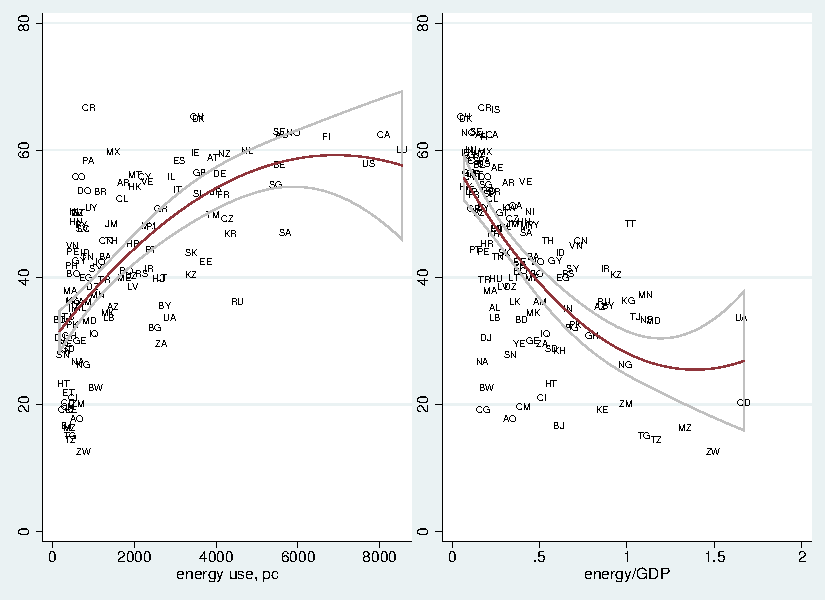
\includegraphics[width=6in]{graphsAndTables/couWdhEneGdpHly.pdf}\centering
\caption{Happy Life Years (HLY) as a dependent variable: An alternative way of
  measuring wellbeing.}\label{hly}
\end{figure}

As a robustness check, it is critical to control for percent urban or population density, because
urban or dense areas are less happy \citep{aokCityBook15} and more energy
efficient \citep{meyer13}, and hence
omission of this variable leads to positive bias on energy use--the estimated
coefficient may be larger than it should be in a bivariate case. Indeed, bivariate
relationship is positive as shown in the paper. 

% The bottom line is that there appears to be weak relationship between electricity
% consumption and happiness, but it disappears or indeed becomes negative when
% taking into account social support. One explanation is that people who consume
% more electricity, need to work more, and have less time for social interaction, which
% is important for happiness. Per Robert Putnam's Bowling Alone, we have less and
% less social interaction and per Robert Frank--we tend to  focus more on non-pecuniary domain!

Regression results are set in table \ref{regA}. First, we start with an ols
model. All ols regressions control for year dummies--different countries
were surveyed in different years. Energy consumption results in greater
happiness (ols1), but when controlling for PCGDP, the relationship disappears
(ols2). Addition of percent urban, unemployment rate and life expectancy (ols3)
makes the relationship actually significantly negative.  Addition of maximum
temperatures in January and July (ols4) makes it positive again but still
insignificant.  A very interesting change  occurs in column ols5--addition of
$CO_2$ makes energy positive and significant.\footnote{The two variables are
  correlated at .91. And coefficient on $CO_2$ is negative as expected. Energy correlates at .38
  with happiness, and $CO_2$ correlates at .29 with happiness ($CO_2$ correlates with development,  hence positive sign).}
 Hence, energy consumption would increase happiness if not emissions. This may
 point to clean energy (wind, solar, etc) as a solution. 

Furthermore, in such a diverse sample of countries, there is some unobserved
heterogeneity. Two fixed effects model follow (temperature drops out, because we
 only have temperature for country for one time period). Yet comfortingly
 results are similar to ols, when not controlling for $CO_2$, results are only weakly
 significant (fe1), but when controlling for $CO_2$,  results become significant
 (fe2). Again, our interpret is that energy consumption WITHOUT pollution would
 contribute to happiness.  But because energy consumption results in pollution,
 it does not contribute to happiness.

\begin{figure}[H]
 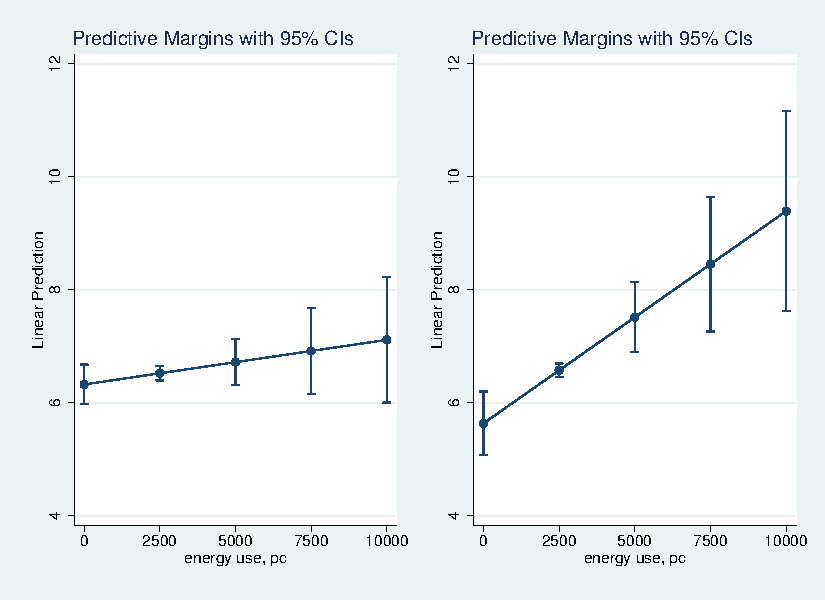
\includegraphics[width=6in]{graphsAndTables/ols4ols5.pdf}\centering
\caption{Predicted probabilities from model  ols4 (first panel); and model ols5
  (second panel)% --the latter controls
  % for co2--if we could have energy without pollution it would increase happiness! 
}\label{ols4ols5}
\end{figure}


\begin{table}[H]\centering \caption{regA} \label{regA} \begin{scriptsize} \begin{tabular}{p{1.4in}p{.43in}p{.43in}p{.43in}p{.43in}p{.43in}p{.43in}p{.43in}p{.43in}p{.43in}p{.43 in}p{.43in}p{.43 in}}\hline                     &        ols1   &        ols2   &        ols3   &        ols4   &        ols5   &         fe1   &         fe2   \\
energy use, pc      &       0.000***&      -0.000+  &      -0.000*  &       0.000   &       0.000** &       0.001+  &       0.001*  \\
PCGDP               &               &       0.000***&       0.000***&       0.000** &       0.000*  &       0.000   &      -0.000   \\
percent urban       &               &               &       0.018** &      -0.001   &      -0.001   &       0.019   &       0.030   \\
unemployment, \%     &               &               &      -0.026*  &      -0.008   &      -0.002   &       0.010   &       0.009   \\
female life expectancy&               &               &       0.006   &       0.050** &       0.057***&      -0.002   &      -0.003   \\
maximum temperature in January&               &               &               &       0.045***&       0.049***&               &               \\
maximum temperature in July&               &               &               &      -0.019*  &      -0.014   &               &               \\
co2 emissions, pc   &               &               &               &               &      -0.108** &               &      -0.262   \\
constant            &       6.592***&       6.693***&       5.473***&       2.725*  &       1.921   &       3.657   &       3.245   \\
N                   &         163   &         162   &         139   &         139   &         139   &         139   &         139   \\
 \hline\multicolumn{6}{l}{+p$<$0.10 *p$<$0.05 **p$<$0.01 ***p$<$0.001; robust standard errors} \end{tabular}\end{scriptsize}\end{table}

\begin{table}[h!]
  \centering\begin{scriptsize}
  \begin{tabular}{lp{.62in}p{.62in}p{.62in}p{.62in}p{.62in}p{.62in}p{.62in}p{.62in}p{.62in}p{.62in}}
             &   energy use, pc &  PCGDP &  percent urban &  unemployment, \% &  female life expectancy & maximum temperature in January& maximum temperature in July&\\\hline
         energy use, pc &   1.0 &      &      &     &       &       &       &\\
         PCGDP &   0.7*&  1.0 &      &     &       &       &       &\\
         percent urban &   0.62*&  0.62*&  1.0 &     &       &       &       &\\
          unemployment, \% &  -0.1*& -0.2*&  0.0 &  1.0&       &       &       &\\
        female life expectancy &   0.62*&  0.62*&  0.7*& -0.0&   1.0 &       &       &\\
      maximum temperature in January &  -0.4*& -0.3*& -0.1 & -0.0&  -0.4*&  1.0  &       &\\
      maximum temperature in July &  -0.3*& -0.3*& -0.3*&  0.0&  -0.2*&  0.2* & 1.0   &\\ 
         co2 emissions, pc &   0.9*&  0.6*&  0.62*& -0.0&   0.4*& -0.4* &-0.2*  &\\
  \end{tabular}\end{scriptsize}
  \caption{Cross-correlation table.}
  \label{ccTab}
\end{table}


\section{US state-level additional results}
How do we use energy in the US? % Energy use is slightly increasing in the US
% (\url{http://www.eia.gov/todayinenergy/detail.cfm?id=4690}), and quite a bit in
% the World. 
Energy use in the US has been fairly flat over past 40 years at 70m btu
pc.(\url{http://www.eia.gov/todayinenergy/detail.cfm?id=3590}), and coasts consume
less than inland middle
(\url{http://energy.gov/maps/2009-energy-consumption-person?page=0%2C1}). 
Use by sector in the US is following: 22\% residential, 18\% commercial, 32\% industrial, and
28\% transportation.(\url{http://www.eia.gov/consumption/}). 


% For the US CBO produced a handy chart (\url{http://www.cbo.gov/publication/43232}) or (\url{http://www.cbo.gov/sites/default/files/43232-infographic-EnergySecurity.pdf})

% Some popular media description
% (\url{http://www.theatlantic.com/technology/archive/2013/08/a-very-short-history-of-how-americans-use-energy-at-home/278329/})

% We know how energy is used in residential sector in the US ( we also know it for
% other sectors but we do not focus on them)--all data are here
% (\url{http://www.eia.gov/forecasts/aeo/MT_residentialdemand.cfm}). For residential
% sector
% (\url{http://www.eia.gov/oiaf/aeo/tablebrowser/aeo_query_server/?event=ehExcel.getFile&study=AEO2014&region=0-0&cases=ref2014-d102413a&table=4-AEO2014&yearFilter=0}):
% table AEO2014: 


%LATER may see footnotes for this table
\begin{table}[H]\centering\footnotesize
\caption{\label{freq_im_god} Total Energy Consumption by End Use; quadrillion
  Btu, 2011.}
\begin{tabular}{lll}   \hline 
Space Heating&	5.6\\
Space Cooling&	2.6\\
Water Heating&	2.7\\
Refrigeration&	1.2\\
Cooking&	0.6\\
Clothes Dryers&	0.7\\
Freezers&	0.2\\
Lighting&	2\\
Clothes Washers&	0.1\\
Dishwashers 1/	0.307437
Televisions and Related Equipment&	1\\
Computers and Related Equipment &	0.4\\
Furnace Fans and Boiler Circulation Pumps&	0.4\\
Other Uses&	3.7\\\hline
\end{tabular}\end{table}

How is electricity used in United States homes? %  This is an important
% consideration because it really shows what we do with this electricity--how we
% consume it, what are the end uses.
Data are shown in table
\ref{eleEndUse}. Furthermore end uses of energy changed over time, for instance
 from 1993 to 2009: appliances share increased from 24\% to 35\% and space
 heating dropped from 53\% to 41\%
 (\url{http://www.eia.gov/todayinenergy/detail.cfm?id=10271&src=%E2%80%B9%20Consumption%20%20%20%20%20%20Residential%20Energy%20Consumption%20Survey%20%28RECS%29-b1}). 
% Also, the good news is that average energy consumption per household dropped from 114 m BTU in 1980 to
% 90 m BTU in 2009 \url{http://www.eia.gov/consumption/residential/reports/2009/consumption-down.cfm?src=%E2%80%B9%20Consumption%20%20%20%20%20%20Residential%20Energy%20Consumption%20Survey%20%28RECS%29-b5}.  


\begin{table}[H]\centering\footnotesize
\caption{\label{eleEndUse}  Estimated U.S. Residential \underline{Electricity} Consumption by End
  Use, 2012 (\url{www.eia.gov/tools/faqs/faq.cfm?id=96&t=3}).}
\begin{tabular} {llll}   \hline 
End Use&Quadrillion Btu &Billion kilowatthours& \% Share of total\\\hline 
Space cooling&0.85&250&18.00\%\\
Lighting&0.64&186&14.00\%\\
Water heating&0.45&130&9.00\%\\
Refrigeration&0.38&111&8.00\%\\
Televisions and related equipment&0.33&98&7.00\%\\
Space heating&0.29&84&6.00\%\\
Clothes dryers&0.2&59&4.00\%\\
Computers and related equipment&0.12&37&3.00\%\\
Cooking&0.11&31&2.00\%\\
Dishwashers &0.1&29&2.00\%\\
Furnace fans and boiler circulation pumps&0.09&28&2.00\%\\
Freezers&0.08&24&2.00\%\\
Clothes washers3&0.03&9&1.00\%\\
Other uses&1.02&299&22.00\%\\\hline
Total consumption&4.69&1375&\\\hline
\end{tabular}\end{table}

% there is also consumption by end use by census region or climate region
% \url{http://www.eia.gov/consumption/residential/data/2009/index.cfm?view=consumption}

% \section{Over-time movement: additional results.}

% \begin{figure}[H]
%  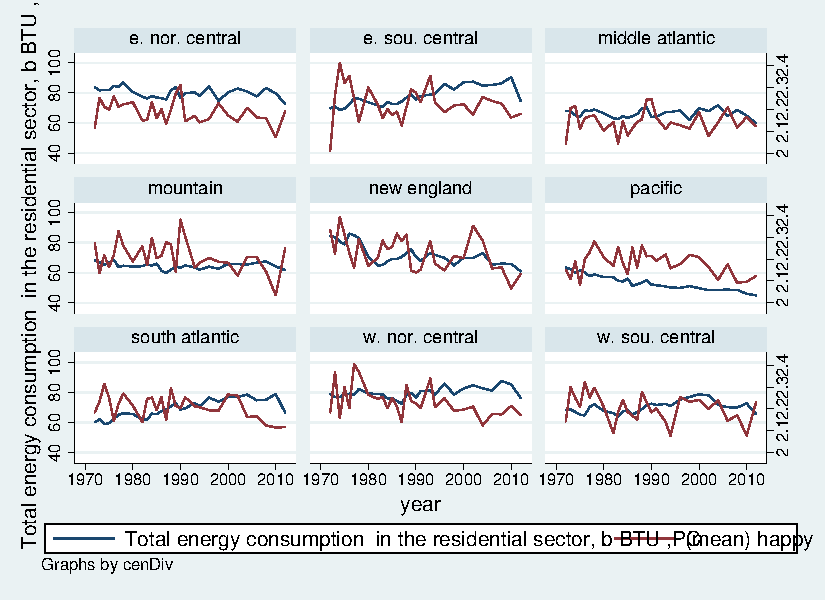
\includegraphics[width=6in]{graphsAndTables/cenDivLsYr.pdf}\centering
% \caption{Happiness and energy use across census divisions over
% time. Unsmoothened series}\label{cenDivLsYr}
%  \end{figure}

% \newpage
% \begin{thebibliography}{10}

% \bibitem{aokCityBook15}
% Okulicz-Kozaryn A (2015) {\em Happiness and Place. Why Life is Better Outside
%   of the City.}
% \newblock (Palgrave Macmillan).

% \bibitem{meyer13}
% Meyer WB (2013) {\em The Environmental Advantages of Cities: Countering
%   Commonsense Antiurbanism}.
% \newblock (MIT Press).
% \end{thebibliography}


\end{spacing}
\end{document}
